% =============================================================================
%  Chapter 9: Recursive and Inductive Types
%  Type Theory from the Ground Up
% =============================================================================

\chapter{Recursive and Inductive Types}
\label{ch:recursive-inductive}

\begin{quote}
\itshape
``To iterate is human, to recurse divine.''
\\ \smallskip
\hspace*{\fill}--- L. Peter Deutsch
\end{quote}

\bigskip

So far in this book we have built up a rich vocabulary of types.
We started with primitive types --- \Bool{}, \Nat{}, \Unit{}, \Void{} --- and
then learned how to combine them: product types (``and''), sum types (``or''),
and function types (``implies'').
In the previous chapter we saw how these operations form a genuine algebra,
with products behaving like multiplication, sums like addition, and functions
like exponentiation.

But there is a glaring omission from that algebra: the data structures you
use every single day.
Linked lists.
Binary trees.
Abstract syntax trees.
JSON values.
File system hierarchies.
Every one of these involves a type that \emph{refers to itself}.

A linked list node contains a value \emph{and} a pointer to another linked
list node.
A binary tree node contains a value and \emph{two} subtrees.
A JSON value is either a number, a string, a boolean, null, an array of JSON
values, or an object mapping strings to JSON values.

This self-reference is what we call \emph{recursion in types}, and handling it
carefully is the subject of this chapter.
We will see that recursive types are not just a hack bolted onto the side of
type theory --- they arise naturally as \emph{fixed points} of type
constructors, they have a beautiful algebraic interpretation, and they come in
two dual flavours: \emph{inductive types} (finite, bottom-up, for data you
construct) and \emph{coinductive types} (potentially infinite, top-down,
for data you observe).

This is a long chapter because the topic is deep, but we will take it one step
at a time.
By the end, the struct definitions you write in C++ every day will look
completely different to you --- you will see them as fixed-point equations,
generators of formal power series, and instances of a general principle
that unifies all of programming.

% =============================================================================
\section{The Problem: Self-Reference in Types}
\label{sec:self-reference}
% =============================================================================

Let us start with the most familiar example.
Here is a singly linked list node in C++:

\begin{lstlisting}[style=cpp]
struct Node {
    int val;
    Node* next;   // <-- a Node contains a pointer to a Node!
};
\end{lstlisting}

Look carefully at what is happening.
The type \typename{Node} is defined in terms of itself: it contains a
\code{Node*} field.
If we try to write this as a type equation using the algebra from Chapter 8,
we get something like:

\[
  \text{Node} = \mathsf{Int} \times \text{Node}
\]

But this is a problem.
If we try to ``solve'' this equation naively, we can substitute
$\text{Node} = \mathsf{Int} \times \text{Node}$ into itself:

\[
  \text{Node}
    = \mathsf{Int} \times (\mathsf{Int} \times (\mathsf{Int} \times (\mathsf{Int} \times \cdots)))
\]

We get an \emph{infinite product} --- a type with infinitely many
$\mathsf{Int}${} fields.
That is not a finite object we can store in memory.

The C++ compiler gets around this by using a \emph{pointer}: \code{Node*}
is not a full \code{Node}, it is an address in memory, and all pointers
have the same size regardless of what they point to.
This is the machine-level hack that makes recursive structs work in C.
But in type theory, we want to understand the \emph{meaning} of these types,
not just their implementation.
And the meaning requires a more careful treatment.

\begin{keyinsight}[The Core Tension]
A type is supposed to be something \emph{finite} we can reason about.
But recursive types appear to be infinitely large.
The resolution: a recursive type is not the infinite unrolling, but the
\emph{fixed point} of a type-level equation.
It is the smallest type that satisfies the equation.
\end{keyinsight}

Before we can solve this, we need to see how to write down the equation
properly.
The key is to separate the ``shape'' of the type from the ``self-reference''.

% =============================================================================
\section{Recursive Type Equations}
\label{sec:recursive-equations}
% =============================================================================

The first step is to write recursive types as \emph{equations}.
This is more than just notation --- it clarifies exactly what we are asking for.

\subsection{Lists}

A list of \code{A} values is either:
\begin{itemize}
  \item empty (the \emph{nil} case), or
  \item an \code{A} value followed by another list of \code{A} values
        (the \emph{cons} case).
\end{itemize}

In type algebra, ``either'' is a sum ($+$), and ``followed by'' is a product
($\times$).
The empty list is a unit-like thing with exactly one inhabitant (the empty
list itself), so it has type $1$ (i.e., \Unit{}).
Writing $L$ for $\text{List}(A)$:

\[
  \boxed{L \;=\; 1 + A \times L}
\]

Read this aloud: ``A list is either the unit type (empty) or a pair of
an \code{A} and another list.''

In Haskell this is written almost verbatim:

\begin{lstlisting}[style=haskell]
data List a = Nil | Cons a (List a)
-- or, using built-in syntax:
data [a] = [] | a : [a]
\end{lstlisting}

\subsection{Binary Trees}

A binary tree of \code{A} values is either:
\begin{itemize}
  \item a leaf (empty), or
  \item a node containing an \code{A} and two subtrees.
\end{itemize}

Writing $T$ for $\text{Tree}(A)$:

\[
  \boxed{T \;=\; 1 + A \times T \times T}
\]

(Here $A \times T \times T$ means a triple: a value and two subtrees.
We use $\times$ as left-associative, so this is $(A \times T) \times T$.)

\begin{lstlisting}[style=haskell]
data Tree a = Leaf | Node a (Tree a) (Tree a)
\end{lstlisting}

\subsection{Natural Numbers}

Natural numbers might surprise you, but they are also a recursive type:

\[
  \boxed{\Nat \;=\; 1 + \Nat}
\]

A natural number is either zero (the unit case) or the successor of a natural
number.
In Haskell (Peano-style):

\begin{lstlisting}[style=haskell]
data Nat = Zero | Succ Nat
-- Zero    represents 0
-- Succ Zero             represents 1
-- Succ (Succ Zero)      represents 2
-- etc.
\end{lstlisting}

\subsection{Rose Trees (n-ary Trees)}

A rose tree is a node containing a value and a \emph{list} of subtrees:

\[
  \text{Rose}(A) = A \times \text{List}(\text{Rose}(A))
\]

This is a \emph{mutually recursive} type: \text{Rose} is defined in terms of
\text{List}, which is itself recursive.

\begin{lstlisting}[style=haskell]
data Rose a = RoseNode a [Rose a]
\end{lstlisting}

\begin{example}[JSON Values]
JSON is a recursive type.
A JSON value is one of:
\begin{align*}
  \text{JSON} \;=\; & \text{Null} \\
               \;+\; & \text{Bool} \\
               \;+\; & \text{Number} \\
               \;+\; & \text{String} \\
               \;+\; & \text{List}(\text{JSON}) \\
               \;+\; & \text{Map}(\text{String}, \text{JSON})
\end{align*}
Where $\text{Null} = 1$, $\text{Bool} = 2$, and $\text{List}$ and $\text{Map}$
are themselves recursive types.
Every JSON parser you have ever written processes this recursive type, whether
or not you thought of it that way.
\end{example}

\begin{intuition}
Recursive type equations say: ``here is the \emph{shape} of the type.''
The equation $L = 1 + A \times L$ does not tell us what $L$ \emph{is} yet
--- it tells us what \emph{structure} $L$ must have.
Finding $L$ means solving this equation in the ``universe'' of types.
\end{intuition}

% =============================================================================
\section{Fixed Points of Type Constructors}
\label{sec:fixed-points}
% =============================================================================

We now have recursive equations like $L = 1 + A \times L$.
What does it mean to ``solve'' such an equation?

The answer comes from the concept of a \emph{fixed point}.

\subsection{Fixed Points, Reviewed}

In ordinary mathematics, a fixed point of a function $f$ is a value $x$
such that $f(x) = x$.
For example, if $f(x) = x^2$, then $f(0) = 0$ and $f(1) = 1$, so $0$ and
$1$ are both fixed points of $f$.

Now think of a recursive type equation $T = F(T)$ where $F$ is some
``type constructor'' (a thing that takes a type and produces a type).
A \emph{type} $T$ that satisfies this equation is a \emph{fixed point} of $F$.

For lists: $F(X) = 1 + A \times X$.
We want the type $L$ such that $F(L) = L$, i.e., $1 + A \times L = L$.

For trees: $F(X) = 1 + A \times X \times X$.
We want the type $T$ such that $F(T) = T$.

For natural numbers: $F(X) = 1 + X$.
We want $\Nat$ such that $1 + \Nat = \Nat$.

\subsection{The \texorpdfstring{$\mu$}{mu} Notation}

Type theorists use a special notation for the fixed point of a type constructor.
The symbol $\mu$ (mu) stands for the \emph{least fixed point}:

\[
  \mu X.\, F(X)
\]

means ``the least fixed point of the type constructor $F$, with $X$ as the
variable representing the recursive occurrence.''

So:

\begin{align*}
  \text{List}(A) &= \mu X.\; 1 + A \times X \\[4pt]
  \text{Tree}(A) &= \mu X.\; 1 + A \times X \times X \\[4pt]
  \Nat           &= \mu X.\; 1 + X
\end{align*}

The variable $X$ in $\mu X. F(X)$ is bound, just like $x$ in $\lambda x. e$:
the name $X$ is just a placeholder for the self-reference.

\begin{keyinsight}[What ``Least'' Means]
Why the \emph{least} fixed point?
In general, $F(X) = X$ might have many solutions.
For type constructors built from $+$, $\times$, and constants, the least fixed
point is the one that contains only \emph{finite}, \emph{explicitly constructed}
values.
It is the smallest type that satisfies the equation.
The least fixed point of $F(X) = 1 + X$ is $\{0, 1, 2, 3, \ldots\}$ (natural
numbers), not the type containing all naturals \emph{plus} an infinite value
``$\omega$''.
We will see the dual (greatest fixed point) when we discuss coinduction.
\end{keyinsight}

\subsection{Unrolling and Rolling}

The equation $T = \mu X.\, F(X)$ means $T \cong F(T)$ (at least up to
isomorphism).
This gives us two operations:

\begin{itemize}
  \item \textbf{Roll} (fold): take an $F(T)$ and produce a $T$.
        This is like calling a constructor.
  \item \textbf{Unroll} (unfold): take a $T$ and produce an $F(T)$.
        This is like pattern matching.
\end{itemize}

For lists, rolling means: given either \Unit{} (empty) or a pair $(a, \ell)$
(cons), produce a list.
Unrolling means: given a list, determine whether it is empty or a cons pair.

In Haskell:

\begin{lstlisting}[style=haskell]
-- Roll:   1 + A * List A  -->  List A
roll :: Either () (a, [a]) -> [a]
roll (Left ())       = []
roll (Right (x, xs)) = x : xs

-- Unroll: List A  -->  1 + A * List A
unroll :: [a] -> Either () (a, [a])
unroll []     = Left ()
unroll (x:xs) = Right (x, xs)
\end{lstlisting}

These two functions are inverses of each other.

% =============================================================================
\section{Iso-recursive vs.\ Equi-recursive Types}
\label{sec:iso-vs-equi}
% =============================================================================

There are two major schools of thought on how to handle recursive types, and
they differ in whether $T$ and $F(T)$ are considered \emph{equal} or merely
\emph{isomorphic}.

\subsection{Equi-recursive Types}

In an \emph{equi-recursive} system, $\mu X.\, F(X)$ is literally
\emph{the same type} as $F(\mu X.\, F(X))$.
You can freely interconvert between them without any explicit operation.

This is the approach taken by Haskell (with its lazy evaluation), most
object-oriented languages, and TypeScript.
You simply write a recursive type and use it without ceremony:

\begin{lstlisting}[style=haskell]
-- Haskell: equi-recursive
-- [a] is literally the same as (Either () (a, [a]))
-- no explicit fold/unfold needed
f :: [Int] -> Int
f []     = 0
f (x:xs) = x + f xs
-- Pattern matching IS the unroll; constructors ARE the roll.
\end{lstlisting}

The theoretical treatment of equi-recursive types requires \emph{coinductive}
reasoning about types (types-as-regular-trees), which is well-developed but
more complex to implement in a type checker.

\subsection{Iso-recursive Types}

In an \emph{iso-recursive} system, $\mu X.\, F(X)$ is
\emph{isomorphic to} $F(\mu X.\, F(X))$, but not definitionally equal.
To convert between them, you need explicit \textbf{fold} and \textbf{unfold}
operations:

\[
  \text{fold}_\mu   : F(\mu X.\, F(X)) \to \mu X.\, F(X)
\]
\[
  \text{unfold}_\mu : \mu X.\, F(X) \to F(\mu X.\, F(X))
\]

These operations have no runtime cost --- they are just type-level annotations
that tell the type checker ``yes, I know I am converting between these
isomorphic types.''

This is the approach taken by most proof assistants (Coq, Agda, Lean), Standard
ML, and implicitly by many type theories.

\begin{cppconnection}[Fold and Unfold in C++]
In C++, constructors and pattern matching (or \code{std::visit}) serve as
fold and unfold.

When you write \code{Node\{42, nullptr\}}, you are folding: converting a
\code{(int, Node*)} pair into a \code{Node}.

When you write:
\begin{lstlisting}[style=cpp]
void process(Node* n) {
    if (n == nullptr) { /* unfold: this is the Nil case */ }
    else              { /* unfold: this is the Cons case; n->val and n->next */ }
}
\end{lstlisting}
you are unfolding: inspecting a \code{Node} to determine which case it is.

The C++ compiler handles this implicitly (the \code{Node*} indirection hides
the recursion), but the logical structure is the same iso-recursive fold/unfold.
\end{cppconnection}

\subsection{Comparison}

\begin{center}
\begin{tabular}{lll}
\toprule
\textbf{Property} & \textbf{Equi-recursive} & \textbf{Iso-recursive} \\
\midrule
$T = F(T)$?       & Definitional equality    & Isomorphism only       \\
Fold/unfold?      & Implicit                 & Explicit               \\
Type checking     & Harder (coinductive)     & Easier                 \\
Used in           & Haskell, TypeScript, OOP & ML, Coq, Agda, Lean    \\
\bottomrule
\end{tabular}
\end{center}

\begin{warning}[Equi-recursive Types and Infinite Loops]
Because equi-recursive types treat $T = F(T)$ as a literal equality, they
can make type checking undecidable if you are not careful.
In particular, without restrictions, you can write types that ``go around in
circles'' during type-checking.
Haskell avoids this by requiring explicit type constructor names
(\typename{data} declarations introduce new, opaque names), which breaks the
cycle at the type-checker level even though the programmer experience feels
like equi-recursion.
\end{warning}

% =============================================================================
\section{Inductive Types}
\label{sec:inductive-types}
% =============================================================================

We now come to the main event: \emph{inductive types}.
An inductive type is a recursive type that is guaranteed to be \emph{finite}.
It is built from the bottom up: you start with base cases and combine them
using constructor rules, and every value can be reached in a finite number
of constructor applications.

This is the type-theoretic formalisation of ``algebraic data types'' in
functional languages.

\subsection{Informal Definition}

An inductive type is specified by:

\begin{enumerate}
  \item A set of \textbf{constructors} (introduction rules): these tell you
        how to \emph{build} values of the type.
  \item An \textbf{elimination principle} (recursion/induction): this tells you
        how to use values of the type, by specifying what to do in each
        constructor case.
\end{enumerate}

\subsection{Natural Numbers as an Inductive Type}

Let us work through natural numbers in detail because they are the simplest
non-trivial example.

\textbf{Constructors (Introduction rules):}
\[
  \frac{}{\vdash \mathtt{zero} : \Nat}
  \qquad\qquad
  \frac{\vdash n : \Nat}{\vdash \mathtt{succ}(n) : \Nat}
\]

Read: (1) \code{zero} is a natural number; (2) if $n$ is a natural number,
then $\code{succ}(n)$ is also a natural number.

\textbf{Elimination rule (the recursion principle):}
To define a function $f : \Nat \to A$ by recursion, you provide:
\begin{itemize}
  \item A base case: $f_0 : A$ (the value of $f$ at \code{zero}).
  \item A step case: $f_s : A \to A$ (given $f(n)$, compute $f(\code{succ}(n))$).
\end{itemize}

\[
  \text{rec}_\Nat : A \to (A \to A) \to \Nat \to A
\]
\[
  \text{rec}_\Nat(f_0, f_s, \mathtt{zero}) = f_0
\]
\[
  \text{rec}_\Nat(f_0, f_s, \mathtt{succ}(n)) = f_s(\text{rec}_\Nat(f_0, f_s, n))
\]

\begin{example}[Addition via Recursion]
\[
  \mathtt{add}(m, n) = \text{rec}_\Nat(n,\; \mathtt{succ},\; m)
\]
\begin{itemize}
  \item Base: $\mathtt{add}(0, n) = n$.
  \item Step: $\mathtt{add}(\mathtt{succ}(m), n) = \mathtt{succ}(\mathtt{add}(m,n))$.
\end{itemize}
\end{example}

\subsection{Lists as an Inductive Type}

\textbf{Constructors:}
\[
  \frac{}{\vdash \mathtt{nil} : \text{List}(A)}
  \qquad\qquad
  \frac{\vdash a : A \quad \vdash \ell : \text{List}(A)}
       {\vdash \mathtt{cons}(a, \ell) : \text{List}(A)}
\]

\textbf{Elimination rule (foldr):}
To define $f : \text{List}(A) \to B$, provide:
\begin{itemize}
  \item A base case $f_\mathtt{nil} : B$.
  \item A step case $f_\mathtt{cons} : A \to B \to B$.
\end{itemize}

\[
  \text{rec}_{\text{List}} : B \to (A \to B \to B) \to \text{List}(A) \to B
\]

This is exactly \code{foldr} in Haskell!

\begin{lstlisting}[style=haskell]
foldr :: b -> (a -> b -> b) -> [a] -> b
foldr base _    []     = base
foldr base step (x:xs) = step x (foldr base step xs)

-- length as a fold:
length' :: [a] -> Int
length' = foldr 0 (\_ acc -> acc + 1)

-- sum as a fold:
sum' :: [Int] -> Int
sum' = foldr 0 (+)

-- map as a fold:
map' :: (a -> b) -> [a] -> [b]
map' f = foldr [] (\x acc -> f x : acc)
\end{lstlisting}

The fact that \code{foldr} is the elimination principle for lists means that
\emph{every} function you can write on lists can be expressed as a fold.
This is a profound unification.

\begin{definition}[Inductive Type]
An \emph{inductive type} $T$ is a type defined by:
\begin{enumerate}
  \item A finite set of \emph{constructors} $c_1, \ldots, c_n$, each of the
        form $c_i : F_i(T) \to T$ for some polynomial type constructor $F_i$.
  \item The \emph{initiality condition}: $T$ is the \emph{initial algebra}
        for these constructors.
        This means: for any other type $X$ with functions $f_i : F_i(X) \to X$,
        there is a unique function $h : T \to X$ that commutes with all
        constructors.
\end{enumerate}
This unique $h$ is the elimination principle (the fold/recursion operator).
\end{definition}

\begin{intuition}
``Initial algebra'' is category-theoretic language, but the intuition is simple:
an inductive type is the \emph{freest} possible type with the given constructors.
It has no other equalities or structure beyond what the constructors impose.
The elimination principle captures exactly the idea ``to process a value of
this type, handle each constructor case.''
\end{intuition}

% =============================================================================
\section{Structural Recursion and Termination}
\label{sec:structural-recursion}
% =============================================================================

One of the most important properties of inductive types is that functions
defined by \emph{structural recursion} always terminate.

\subsection{What is Structural Recursion?}

A function is defined by \emph{structural recursion} on an inductive type if:
\begin{itemize}
  \item It is defined by cases on the constructors of the type.
  \item Every recursive call is on a \emph{structurally smaller} argument ---
        i.e., an argument that was obtained by pattern matching (``one layer
        peeled off'').
\end{itemize}

\begin{example}[List Length]
\begin{lstlisting}[style=haskell]
length :: [a] -> Int
length []     = 0               -- base case: Nil
length (_:xs) = 1 + length xs  -- recursive case: xs is smaller than (x:xs)
\end{lstlisting}

The argument to the recursive call, \code{xs}, is the tail of the input
\code{(x:xs)}.
It is \emph{structurally smaller}: it was produced by pattern matching.
So this function is structurally recursive and definitely terminates.
\end{example}

\begin{example}[Tree Size]
\begin{lstlisting}[style=haskell]
data Tree a = Leaf | Node a (Tree a) (Tree a)

size :: Tree a -> Int
size Leaf         = 0
size (Node _ l r) = 1 + size l + size r
-- Both l and r are structurally smaller than (Node _ l r)
\end{lstlisting}
\end{example}

\begin{example}[Addition on Peano Naturals]
\begin{lstlisting}[style=haskell]
add :: Nat -> Nat -> Nat
add Zero     n = n
add (Succ m) n = Succ (add m n)
-- In the recursive call, m is structurally smaller than (Succ m)
\end{lstlisting}
\end{example}

\subsection{Why Structural Recursion Always Terminates}

The key insight is that inductive types have a \emph{well-founded} structure.
Every value is built from constructors in a finite number of steps.
When you pattern match, you get a strictly smaller value (fewer constructor
layers).
Since you cannot peel off infinitely many layers from a finite structure,
the recursion must eventually reach a base case.

\begin{keyinsight}[Structural Recursion = Termination for Free]
If your function is defined by structural recursion on an inductive type, you
get termination for free --- no need for complex termination proofs.
This is one of the core reasons type theory and proof assistants insist on
structural recursion: if every function terminates, the logic is consistent
(you cannot prove \Void{} by an infinite loop).
\end{keyinsight}

\subsection{The Induction Principle}

Structural recursion has a logical counterpart: the \emph{induction principle}.
For natural numbers, the recursion principle says:

\textit{To prove that a property $P$ holds for all natural numbers, prove:
\begin{enumerate}
  \item $P(\text{zero})$ (the base case), and
  \item For all $n$, if $P(n)$ then $P(\text{succ}(n))$ (the inductive step).
\end{enumerate}}

This is just structural recursion, but ``into $\text{Prop}$'' (the universe of
propositions) rather than into a data type.

For lists:

\textit{To prove $P$ for all lists, prove:
\begin{enumerate}
  \item $P(\text{nil})$, and
  \item For all $x$ and $\ell$, if $P(\ell)$ then $P(\text{cons}(x, \ell))$.
\end{enumerate}}

The unification of \emph{computation} (recursion) and \emph{reasoning}
(induction) is the Curry-Howard correspondence in action:
the recursion principle \emph{is} the induction principle, just used for
different purposes.

\begin{cppconnection}[Structural Recursion in C++]
C++ does not enforce structural recursion, but the pattern is common.
Any function that pattern-matches on a recursive data type and only recurses on
sub-components follows the pattern:

\begin{lstlisting}[style=cpp]
// A recursive linked list
struct List {
    int head;
    List* tail;   // nullptr means Nil
};

// Structural recursion: recurse only on tail (structurally smaller)
int length(const List* lst) {
    if (lst == nullptr) return 0;           // base case
    return 1 + length(lst->tail);          // recursive call on tail
}

int sum(const List* lst) {
    if (lst == nullptr) return 0;
    return lst->head + sum(lst->tail);
}
\end{lstlisting}

In C++, the compiler does not verify that your recursion is structural ---
you could recurse on \code{lst} itself and loop forever.
Proof assistants like Agda and Coq enforce structural recursion and reject
non-terminating functions.
\end{cppconnection}

% =============================================================================
\section{The Algebra of Recursive Types}
\label{sec:algebra-recursive}
% =============================================================================

Now we come to one of the most beautiful parts of this chapter: the
\emph{algebraic} interpretation of recursive types.
In Chapter 8 we saw that types form a semiring: product is multiplication,
sum is addition.
What happens when we extend this algebra with the $\mu$ fixed point?

\subsection{Solving the List Equation}

Recall: $L = 1 + A \cdot L$.
Let us treat this like an algebraic equation and solve for $L$:

\[
  L = 1 + A \cdot L
\]
\[
  L - A \cdot L = 1
\]
\[
  L \cdot (1 - A) = 1
\]
\[
  L = \frac{1}{1 - A}
\]

Now expand $\frac{1}{1-A}$ as a geometric series (valid when $|A| < 1$):

\[
  L = \frac{1}{1-A} = 1 + A + A^2 + A^3 + \cdots
\]

In type-theoretic terms:

\[
  \text{List}(A) = 1 + A + A^2 + A^3 + \cdots
\]

This says: a list is either empty ($1$), or a 1-element list ($A$), or a
2-element list ($A^2 = A \times A$), or a 3-element list ($A^3$), and so on.

\textbf{This is exactly right.}
A list of $A$ is exactly a list of zero or more $A$ values, which is the
sum of ``exactly $k$ elements'' over all $k \geq 0$.

\begin{keyinsight}[Lists as Formal Power Series]
The type $\text{List}(A) = \sum_{k=0}^{\infty} A^k$ is not just a metaphor.
If $A$ is a type with $|A| = n$ elements, then:
\[
  |\text{List}(A)| = \sum_{k=0}^{\infty} n^k = \frac{1}{1-n}
\]
Formally divergent, of course (for $n \geq 1$), but the \emph{generating function}
perspective is what makes it meaningful: each term $n^k$ counts the lists
of exactly $k$ elements, and the sum counts all lists.
This is the generating function for sequences: $\frac{1}{1-x}$ at $x = n$.
\end{keyinsight}

\subsection{The Catalan Numbers and Binary Trees}

Binary trees: $T = 1 + A \cdot T^2$.
Treat this as a quadratic equation in $T$:

\[
  T = 1 + A \cdot T^2
\]
\[
  A \cdot T^2 - T + 1 = 0
\]

Using the quadratic formula:

\[
  T = \frac{1 \pm \sqrt{1 - 4A}}{2A}
\]

Expanding $\sqrt{1-4A}$ as a power series and taking the ``small'' solution
(the least fixed point), we get:

\[
  T = \sum_{n=0}^{\infty} C_n \cdot A^n
\]

where $C_n = \frac{1}{n+1}\binom{2n}{n}$ are the \textbf{Catalan numbers}!

The Catalan numbers count the number of binary trees with $n$ internal nodes:
$C_0 = 1$ (one empty tree), $C_1 = 1$ (one tree with one node), $C_2 = 2$
(two trees with two nodes), $C_3 = 5$, $C_4 = 14$, etc.

\begin{example}[Why $C_2 = 2$?]
Binary trees with 2 internal nodes:
\begin{center}
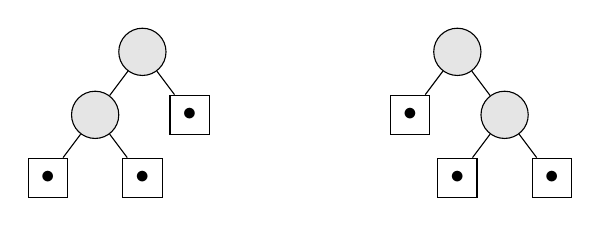
\begin{tikzpicture}[
  node/.style={circle,draw,fill=gray!20,minimum size=6mm,inner sep=1pt},
  leaf/.style={rectangle,draw,fill=white,minimum size=5mm,inner sep=1pt},
  level distance=8mm,
  sibling distance=12mm
]
% Tree 1: left-leaning
\begin{scope}[xshift=-2cm]
  \node[node] {}
    child { node[node] {}
      child { node[leaf] {$\bullet$} }
      child { node[leaf] {$\bullet$} }
    }
    child { node[leaf] {$\bullet$} };
\end{scope}
% Tree 2: right-leaning
\begin{scope}[xshift=2cm]
  \node[node] {}
    child { node[leaf] {$\bullet$} }
    child { node[node] {}
      child { node[leaf] {$\bullet$} }
      child { node[leaf] {$\bullet$} }
    };
\end{scope}
\end{tikzpicture}
\end{center}
There are exactly 2 such trees, matching $C_2 = 2$.
\end{example}

\begin{keyinsight}[The Combinatorial Miracle]
The fact that the type-algebraic equation for binary trees, solved formally
as a polynomial equation, gives the Catalan numbers is not a coincidence.
It reflects a deep connection between type theory, combinatorics, and the theory
of algebraic data types.
The ``type'' of binary trees literally \emph{is} the generating function
for Catalan numbers, and formal manipulation of type equations gives you
combinatorial identities.
This area of research is called \emph{species theory} (Joyal, 1981) and
\emph{dissection} in combinatorics.
\end{keyinsight}

\subsection{Differentiation of Types}

There is one more astonishing result.
In Chapter 8 we mentioned that the ``derivative'' of a type $F$ with respect
to $A$, written $\partial_A F$, is the type of ``one-hole contexts'' for $F$ ---
the type of $F$-structures with one $A$ slot removed (a ``zipper'').

For lists:
\[
  \frac{\partial}{\partial A} \text{List}(A)
  = \frac{\partial}{\partial A} \frac{1}{1-A}
  = \frac{1}{(1-A)^2}
  = \text{List}(A)^2
\]

A list zipper (one-hole context) is a pair of lists: everything before the
hole, and everything after.
The derivative of the list type gives exactly this!

For binary trees:
\[
  \frac{\partial}{\partial A} \text{Tree}(A)
  = \text{List}(\text{Tree}(A) \times \text{Tree}(A))
\]

A tree zipper is a list of ``contexts'' needed to navigate from root to a hole,
each context recording the two subtrees at each level.
The algebra predicts this correctly.

% =============================================================================
\section{Pattern Matching as Elimination}
\label{sec:pattern-matching}
% =============================================================================

Pattern matching is not just convenient syntax.
It \emph{is} the elimination principle for inductive types, and understanding
this connection deepens your understanding of both.

\subsection{Pattern Matching and the Universal Property}

The elimination principle for \text{List}(A) says:
given handlers for each constructor, produce a function from lists to any type.
In Haskell, this is written by listing cases:

\begin{lstlisting}[style=haskell]
-- Explicit elimination:
elim :: b -> (a -> [a] -> b) -> [a] -> b
elim base step []     = base
elim base step (x:xs) = step x xs

-- Pattern matching is sugar for this:
f :: [Int] -> Int
f []     = 0
f (x:xs) = x + f xs

-- Which desugars to:
f = elim 0 (\x xs -> x + f xs)
\end{lstlisting}

\subsection{Pattern Matching in C++ with \code{std::variant}}

In C++, the closest equivalent to inductive types is \code{std::variant},
and the elimination principle is \code{std::visit}:

\begin{lstlisting}[style=cpp]
#include <variant>
#include <functional>
#include <memory>

// Represents: List(int) = 1 + int * List(int)
struct Nil {};
struct Cons;
using List = std::variant<Nil, std::shared_ptr<Cons>>;

struct Cons {
    int head;
    List tail;
};

// Elimination: std::visit acts as the fold
int length(const List& lst) {
    return std::visit([](auto&& arg) -> int {
        using T = std::decay_t<decltype(arg)>;
        if constexpr (std::is_same_v<T, Nil>) {
            return 0;                             // base case
        } else {
            return 1 + length(arg->tail);         // recursive case
        }
    }, lst);
}

int sum_list(const List& lst) {
    return std::visit([](auto&& arg) -> int {
        using T = std::decay_t<decltype(arg)>;
        if constexpr (std::is_same_v<T, Nil>) {
            return 0;
        } else {
            return arg->head + sum_list(arg->tail);
        }
    }, lst);
}
\end{lstlisting}

\begin{cppconnection}[Expression Trees and ASTs]
One of the most common uses of recursive types in C++ is expression trees
(Abstract Syntax Trees).
Every compiler or interpreter you write uses this pattern:

\begin{lstlisting}[style=cpp]
#include <variant>
#include <memory>
#include <string>

struct Num    { double value; };
struct Var    { std::string name; };
struct Add;
struct Mul;
struct IfPos;

using Expr = std::variant<
    Num,
    Var,
    std::shared_ptr<Add>,
    std::shared_ptr<Mul>,
    std::shared_ptr<IfPos>
>;

struct Add    { Expr left; Expr right; };
struct Mul    { Expr left; Expr right; };
struct IfPos  { Expr cond; Expr then_; Expr else_; };

// Evaluate an expression
// This is structural recursion on the Expr inductive type
double eval(const Expr& e, const auto& env) {
    return std::visit([&](auto&& node) -> double {
        using T = std::decay_t<decltype(node)>;
        if constexpr (std::is_same_v<T, Num>)
            return node.value;
        else if constexpr (std::is_same_v<T, Var>)
            return env.at(node.name);
        else if constexpr (std::is_same_v<T, std::shared_ptr<Add>>)
            return eval(node->left, env) + eval(node->right, env);
        else if constexpr (std::is_same_v<T, std::shared_ptr<Mul>>)
            return eval(node->left, env) * eval(node->right, env);
        else if constexpr (std::is_same_v<T, std::shared_ptr<IfPos>>)
            return eval(node->cond, env) > 0
                   ? eval(node->then_, env)
                   : eval(node->else_, env);
    }, e);
}
\end{lstlisting}

The type of \code{Expr} is the type equation:
\[
  \text{Expr} = \text{Num} + \text{Var} + \text{Expr} \times \text{Expr}
                + \text{Expr} \times \text{Expr}
                + \text{Expr} \times \text{Expr} \times \text{Expr}
\]
and \code{eval} is the fold/elimination over this inductive type.
\end{cppconnection}

\subsection{The Correspondence Table}

\begin{center}
\begin{tabular}{lll}
\toprule
\textbf{Type Theory}       & \textbf{Haskell}       & \textbf{C++} \\
\midrule
Constructor (intro rule)   & Data constructor        & Struct constructor / make \\
Elimination principle      & Pattern matching        & \code{std::visit} / if-else \\
Base case                  & Nullary constructor     & Empty variant case \\
Recursive case             & Constructor with args   & Nested variant case \\
Structural recursion       & Recursive function      & Recursive \code{std::visit} \\
Fold                       & \code{foldr}            & Recursive visitor \\
\bottomrule
\end{tabular}
\end{center}

% =============================================================================
\section{Recursive Types in C++: Self-referential Templates and CRTP}
\label{sec:recursive-cpp}
% =============================================================================

C++ has its own idiosyncratic ways of expressing recursive and self-referential
types, some of which are used heavily in practice.

\subsection{Self-referential Struct Templates}

The straightforward case: a struct that contains a pointer to itself,
parameterised by element type.

\begin{lstlisting}[style=cpp]
template<typename T>
struct Node {
    T val;
    Node<T>* next;   // pointer to Node<T>: the recursive occurrence

    Node(T v, Node<T>* n = nullptr) : val(v), next(n) {}
};

template<typename T>
struct BinaryTree {
    T val;
    BinaryTree<T>* left;
    BinaryTree<T>* right;

    BinaryTree(T v,
               BinaryTree<T>* l = nullptr,
               BinaryTree<T>* r = nullptr)
        : val(v), left(l), right(r) {}
};
\end{lstlisting}

In type-equation terms:
\[
  \text{Node}(T) = T \times \text{Node}(T)^?
\]
where ``$?$'' means ``nullable pointer''.
A nullable pointer to $T$ is isomorphic to $1 + T$, so:
\[
  \text{Node}(T) = T \times (1 + \text{Node}(T))
  \;=\; T + T \times \text{Node}(T)
\]
This is the non-empty list equation.
A non-empty list of $T$ is either a single $T$, or a $T$ followed by another
non-empty list.

\subsection{CRTP: The Curiously Recurring Template Pattern}

CRTP is one of the most mind-bending patterns in C++, and it is a perfect
example of a type that refers to itself at the type level:

\begin{lstlisting}[style=cpp]
// Base class is parameterised by the DERIVED class itself!
template<typename Derived>
class Base {
public:
    void interface() {
        // Downcast to Derived and call the implementation
        static_cast<Derived*>(this)->implementation();
    }

    // Default implementation (can be overridden)
    void implementation() {
        // ...
    }
};

// Derived passes itself as the template argument to Base
class MyClass : public Base<MyClass> {
public:
    void implementation() {
        // MyClass-specific implementation
        std::cout << "MyClass::implementation\n";
    }
};

// Usage: static polymorphism, no virtual dispatch
MyClass obj;
obj.interface();  // calls MyClass::implementation() statically
\end{lstlisting}

\textbf{Why is this mind-bending?}
\code{Base<MyClass>} contains a reference to \code{MyClass}, but
\code{MyClass} inherits from \code{Base<MyClass>}.
So the type of the base class \emph{refers to the derived class}, which is
exactly self-reference at the type level.

\begin{keyinsight}[CRTP as a Fixed-Point Type]
CRTP defines a type $D$ such that $D \supseteq \text{Base}(D)$:
$D$ extends (contains) $\text{Base}(D)$.
This is a type-level fixed point equation: $D = \text{Base}(D) + \text{extra}$.

In type theory, this corresponds to a \emph{coinductive} or \emph{recursive}
type where the ``recursion'' is in the \emph{interface}, not just the data.
CRTP achieves static polymorphism by resolving this self-reference at compile
time (since template instantiation knows the concrete type), whereas
\code{virtual} resolves it at runtime.
\end{keyinsight}

\begin{lstlisting}[style=cpp]
// A more sophisticated CRTP example: the "clone" pattern
template<typename Derived>
class Cloneable {
public:
    std::unique_ptr<Derived> clone() const {
        return std::make_unique<Derived>(
            static_cast<const Derived&>(*this)
        );
    }
};

class Document : public Cloneable<Document> {
public:
    std::string content;
    explicit Document(std::string c) : content(std::move(c)) {}
};

// Usage
Document doc("Hello, World!");
auto copy = doc.clone();  // returns unique_ptr<Document>
\end{lstlisting}

\begin{lstlisting}[style=cpp]
// CRTP for static polymorphism / "mixin" functionality:
// Expression template example (a common use in numerics libraries)
template<typename Derived>
struct Expr {
    double eval() const {
        return static_cast<const Derived*>(this)->eval_impl();
    }
};

struct Constant : Expr<Constant> {
    double val;
    explicit Constant(double v) : val(v) {}
    double eval_impl() const { return val; }
};

template<typename L, typename R>
struct Sum : Expr<Sum<L,R>> {
    L left; R right;
    Sum(L l, R r) : left(l), right(r) {}
    double eval_impl() const {
        return left.eval() + right.eval();
    }
};

// The type Sum<Constant, Constant> is an inductive expression type,
// but evaluated statically at compile time with no virtual dispatch.
auto expr = Sum(Constant(3.0), Constant(4.0));
double result = expr.eval();  // = 7.0, all inlined at compile time
\end{lstlisting}

% =============================================================================
\section{Coinductive Types and Codata}
\label{sec:coinductive}
% =============================================================================

We have been discussing \emph{inductive} types: types built from the ground up,
with finite values, using \emph{constructors}.
Now we turn to their dual: \emph{coinductive} types.

\subsection{The Dual Perspective}

Inductive types are characterised by:
\begin{itemize}
  \item Values are \emph{built} by applying constructors.
  \item All values are \emph{finite}.
  \item Functions on them are defined by \emph{structural recursion} (consuming data).
  \item They are \emph{initial algebras}: least fixed points.
\end{itemize}

Coinductive types are the mirror image:
\begin{itemize}
  \item Values are \emph{observed} by applying destructors (projections).
  \item Values can be \emph{infinite}.
  \item Functions into them are defined by \emph{corecursion} (producing data).
  \item They are \emph{final coalgebras}: greatest fixed points.
\end{itemize}

\subsection{Streams: The Prototypical Coinductive Type}

An infinite stream of \code{A} values is defined by:

\[
  \text{Stream}(A) = A \times \text{Stream}(A)
\]

Notice: \emph{no base case}.
A stream always has a head (an \code{A}) and a tail (another stream).
This is the \emph{greatest fixed point} $\nu$:

\[
  \text{Stream}(A) = \nu X.\; A \times X
\]

You cannot build a stream by induction (from the bottom up) because there is
no base case to start from.
Instead, you define a stream by \emph{corecursion}: specify how to produce
the next element given the current state.

\begin{lstlisting}[style=haskell]
-- Haskell's lazy lists ARE coinductive streams
-- They can be infinite because Haskell is lazy

-- The infinite stream of natural numbers
nats :: [Integer]
nats = 0 : map (+1) nats
-- nats = [0, 1, 2, 3, 4, ...]

-- The Fibonacci stream
fibs :: [Integer]
fibs = 0 : 1 : zipWith (+) fibs (tail fibs)
-- fibs = [0, 1, 1, 2, 3, 5, 8, 13, ...]

-- Corecursion: define a stream by specifying the production rule
unfold :: (b -> (a, b)) -> b -> [a]
unfold step seed =
    let (x, next) = step seed
    in x : unfold step next

-- Natural numbers via unfold
nats' :: [Integer]
nats' = unfold (\n -> (n, n+1)) 0
\end{lstlisting}

The function \code{unfold} (also called \code{unfoldr} or \code{anamorphism})
is the \emph{introduction principle} for streams:
to create a stream, provide a seed and a step function.
This is dual to \code{foldr} (the \emph{elimination principle} for lists).

\subsection{Greatest Fixed Points: $\nu$}

The notation $\nu X.\, F(X)$ denotes the \emph{greatest fixed point} of $F$.

\begin{align*}
  \text{Stream}(A) &= \nu X.\; A \times X \\
  \text{InfTree}(A) &= \nu X.\; A \times X \times X
    \quad\text{(infinite binary trees)} \\
  \text{Proc}(S, A) &= \nu X.\; S \to A \times X
    \quad\text{(a process consuming state and producing output)}
\end{align*}

The greatest fixed point of $F(X) = 1 + A \times X$ is not the finite lists
$\mu X.\, 1 + A \times X$ but rather the type of \emph{lazy lists}: either
empty or a pair of an element and a (possibly infinite) rest.

\begin{center}
\begin{tabular}{lll}
\toprule
              & \textbf{Inductive ($\mu$)} & \textbf{Coinductive ($\nu$)} \\
\midrule
Fixed point   & Least                      & Greatest \\
Values        & Finite                     & Possibly infinite \\
Construction  & Constructors (intro)        & Corecursion / unfold \\
Observation   & Pattern match / fold        & Destructors (projections) \\
Haskell analog & \code{data} (strict)       & \code{data} with laziness \\
Termination   & Always terminates          & Productivity (always makes progress) \\
\bottomrule
\end{tabular}
\end{center}

\begin{intuition}
Inductive types answer the question: ``what \emph{is} this value?''
You build it up from constructors and can exhaustively describe it.

Coinductive types answer the question: ``what can I \emph{do} with this value?''
You observe it through projections.
An infinite stream is never ``done'' --- you can always ask for the next element.

An analogy: a \emph{book} is inductive (a finite sequence of pages, you can
read it all). An \emph{ongoing conversation} is coinductive (it produces more
content whenever you participate).
\end{intuition}

\subsection{Corecursion and Productivity}

For inductive types, the safety condition is \emph{termination}: every
recursive call is on a smaller argument.

For coinductive types, the dual condition is \emph{productivity}: every
corecursive definition must make progress.
In each step, it must produce at least one constructor before making the
recursive call.

\begin{lstlisting}[style=haskell]
-- PRODUCTIVE: produces one element (:) before recurring
ones :: [Int]
ones = 1 : ones     -- productive; equivalent to 1 : 1 : 1 : ...

-- PRODUCTIVE: zipWith produces one element before both recursive calls
fibs :: [Integer]
fibs = 0 : 1 : zipWith (+) fibs (tail fibs)

-- Would NOT be productive (in a strict setting):
-- bad = bad   -- makes no progress; pure infinite loop
\end{lstlisting}

Proof assistants that handle coinduction (Coq, Agda) check productivity just
as they check termination for induction.

\begin{cppconnection}[Lazy Evaluation and Coroutines in C++]
C++ is strict (eager) by default, so you cannot write infinite data structures
directly.
But C++20 coroutines provide a way to express coinductive/corecursive
computations:

\begin{lstlisting}[style=cpp]
#include <coroutine>
#include <cstdint>

// A simple generator (lazy stream)
template<typename T>
struct Generator {
    struct promise_type {
        T current_value;
        auto get_return_object() {
            return Generator{
                std::coroutine_handle<promise_type>::from_promise(*this)
            };
        }
        std::suspend_always initial_suspend() { return {}; }
        std::suspend_always final_suspend() noexcept { return {}; }
        std::suspend_always yield_value(T value) {
            current_value = value;
            return {};
        }
        void return_void() {}
        void unhandled_exception() {}
    };

    std::coroutine_handle<promise_type> handle;

    ~Generator() { if (handle) handle.destroy(); }
    T next() { handle.resume(); return handle.promise().current_value; }
};

// Infinite stream of natural numbers (coinductive!)
Generator<uint64_t> naturals() {
    uint64_t n = 0;
    while (true) co_yield n++;   // productive: yields one value per step
}

// Usage: observe the first 10 elements
auto gen = naturals();
for (int i = 0; i < 10; ++i)
    std::cout << gen.next() << " ";
// Output: 0 1 2 3 4 5 6 7 8 9
\end{lstlisting}

A C++20 generator is a coinductive type: it does not contain all the values
(that would require infinite memory), but it can \emph{produce} any value on
demand.
This is exactly the coinductive ``greatest fixed point'' perspective:
you observe one element at a time.
\end{cppconnection}

% =============================================================================
\section{W-Types: The General Form of Inductive Types}
\label{sec:w-types}
% =============================================================================

We have seen many specific inductive types: naturals, lists, trees, ASTs.
Is there a single, unified description that captures all of them?
The answer is yes: \emph{W-types} (well-founded trees, or well-order types).

\subsection{What is a W-type?}

A W-type is parameterised by two pieces of data:

\begin{itemize}
  \item $A : \Type$ --- the type of \emph{constructor labels} (the ``which
        constructor?'' information).
  \item $B : A \to \Type$ --- for each constructor label $a : A$, the type
        $B(a)$ of its \emph{recursive argument positions}.
\end{itemize}

The W-type is written $\mathsf{W}(a : A).\, B(a)$ or simply $\mathsf{W}_{a:A} B(a)$.

An element of $\mathsf{W}_{a:A} B(a)$ is a \emph{well-founded tree}:
a node labelled by some $a : A$, with one subtree for each element of $B(a)$.

\subsection{Examples}

\textbf{Natural numbers:}
Let $A = \{0, 1\}$ (two constructors: Zero and Succ), and:
\[
  B(0) = \Void \quad (\text{Zero has no recursive arguments})
\]
\[
  B(1) = \Unit \quad (\text{Succ has exactly one recursive argument})
\]

A natural number is a tree where each node is either labelled $0$ (a leaf,
no subtrees) or labelled $1$ (one subtree).
This is exactly the Peano naturals.

\textbf{Binary trees over $A$:}
Let $C = \{\mathtt{leaf}, \mathtt{node}\}$, and:
\[
  B(\mathtt{leaf}) = \Void
\]
\[
  B(\mathtt{node}) = \text{Bool} \quad
    (\text{two recursive arguments: left and right, indexed by } \text{Bool})
\]

A value is a tree where leaves have no subtrees and nodes have exactly two
subtrees (one for \code{true}, one for \code{false}).

\textbf{Lists over $A$:}
Let $C = \{\mathtt{nil}\} + A$ (nil constructor, plus one constructor per
element $a : A$), and:
\[
  B(\mathtt{nil}) = \Void
\]
\[
  B(a) = \Unit \quad \text{for each } a : A
\]

A value is a tree where each node is either a nil (leaf) or labelled by an
element $a$ with one subtree (the tail).

\subsection{The Elimination Principle for W-types}

The elimination principle says: to define a function $f : \mathsf{W}_{a:A} B(a) \to C$,
provide a step function:

\[
  \text{step} : \prod_{a:A} (B(a) \to C) \to C
\]

Given a constructor label $a$ and the results of recursing on all subtrees,
produce a $C$.

\begin{keyinsight}[W-types Unify All Inductive Types]
Every inductive type you can write in Haskell or a proof assistant can be
encoded as a W-type.
W-types are to inductive types what sum/product types are to algebraic data
types: a universal primitive from which everything else can be built.

Concretely, $A$ is the disjoint union of all constructor names, and
$B(a)$ is the number/type of recursive positions for constructor $a$.
Non-recursive fields are encoded as additional data attached to the label.

Proof assistants like Agda, Coq, and Lean use W-types (or closely related
constructs like strictly positive types) as their theoretical foundation for
inductive types.
\end{keyinsight}

\begin{definition}[W-type Introduction]
The introduction rule for W-types: given $a : A$ and $f : B(a) \to \mathsf{W}_{a:A} B(a)$
(the subtrees), we can form:
\[
  \mathsf{sup}(a, f) : \mathsf{W}_{a:A} B(a)
\]
This is the single constructor for all W-types.
Every other inductive type's constructors decompose into this form.
\end{definition}

\subsection{Why This Matters}

Even if you never use W-types directly, knowing they exist is important for
three reasons:

\begin{enumerate}
  \item \textbf{Justification}: It tells you that a language with sum types,
        product types, function types, and W-types can express any computable
        inductive structure.
        You do not need to add bespoke recursion mechanisms for every new data
        type.
  \item \textbf{Metatheory}: Proofs about type systems can be done by reducing
        inductive types to W-types, then proving properties of W-types once.
  \item \textbf{Homotopy Type Theory (HoTT)}: In modern type theory, inductive
        types are studied in terms of their \emph{elimination principles}
        (higher inductive types), and W-types are one window into this.
\end{enumerate}

% =============================================================================
\section{Putting It All Together: A Unified View}
\label{sec:unified-view}
% =============================================================================

We have covered a lot of ground.
Let us draw everything together into a unified picture.

\subsection{The Landscape of Recursive Types}

\begin{center}
\begin{tikzpicture}[
  box/.style={rectangle, draw, rounded corners, minimum width=3.5cm,
              minimum height=1cm, align=center, font=\small},
  arrow/.style={-{Stealth}, thick},
  note/.style={font=\footnotesize\itshape, align=center}
]

% Main concepts
\node[box, fill=blue!10]  (inductive)  at (0, 4)    {Inductive Types \\ $\mu X. F(X)$};
\node[box, fill=green!10] (coinductive) at (6, 4)   {Coinductive Types \\ $\nu X. F(X)$};
\node[box, fill=yellow!10] (wtype)     at (0, 1.5)  {W-Types};
\node[box, fill=orange!10] (algebra)   at (6, 1.5)  {Type Algebra \\ (Ch.\ 8)};
\node[box, fill=purple!10] (fixpoint)  at (3, 6)    {Fixed Points \\ of Functors};

% Arrows
\draw[arrow] (fixpoint) -- node[left,  note] {least}    (inductive);
\draw[arrow] (fixpoint) -- node[right, note] {greatest}  (coinductive);
\draw[arrow] (inductive)  -- node[left,  note] {special case}  (wtype);
\draw[arrow] (algebra)    -- node[below, note] {extended with $\mu$} (inductive);
\draw[arrow] (inductive)  -- node[below, note] {dual}     (coinductive);

% Labels at the sides
\node[note] at (-2.5, 4)   {Finite data \\ Bottom-up \\ Constructors \\ Fold/Recur};
\node[note] at (9.2, 4)    {Infinite data \\ Top-down \\ Destructors \\ Unfold/Corec};
\node[note] at (-2.5, 1.5) {Most general \\ Every inductive \\ type encodes here};
\node[note] at (9.2, 1.5)  {$+, \times, \to$ \\ power series \\ Catalan numbers};

\end{tikzpicture}
\end{center}

\subsection{The Full List Hierarchy}

Lists provide a perfect example of the range of recursive types:

\begin{itemize}
  \item \textbf{Finite list} ($\mu X.\, 1 + A \times X$):
        the standard inductive list.
        Values: $[], [1], [1,2], [1,2,3], \ldots$

  \item \textbf{Infinite stream} ($\nu X.\, A \times X$):
        the coinductive stream, no base case.
        Values: $[1, 1, 1, \ldots], [0, 1, 2, 3, \ldots], \ldots$

  \item \textbf{Lazy list} ($\nu X.\, 1 + A \times X$):
        the greatest fixed point of the list functor.
        Values: any finite list, plus any infinite list.
        This is Haskell's \code{[a]}.

  \item \textbf{Non-empty list} ($\mu X.\, A \times (1 + X)$):
        at least one element.
        Also written \code{NonEmpty a} in Haskell.
\end{itemize}

\begin{warning}[Haskell's Types are Lazily Recursive]
In Haskell, \code{data [a] = [] | a : [a]} defines what looks like an
inductive type (finite lists), but Haskell's lazy evaluation makes it actually
the \emph{greatest} fixed point --- lazy lists.
You can write \code{ones = 1 : ones} and it is a perfectly valid value.
If you want genuinely finite, strict lists, you need to work with strict data
or use libraries like \code{Data.Sequence}.

This is one reason Haskell is sometimes called a ``lazily typed'' language in
the informal sense: its types look inductive but behave coinductively.
\end{warning}

% =============================================================================
\section{Summary}
\label{sec:summary-ch9}
% =============================================================================

This chapter has taken us from the ad hoc self-referential struct to a complete
formal theory of recursive types.
Let us recap the key ideas.

\textbf{Recursive type equations.}
Every recursive type can be written as an equation $T = F(T)$ for some
type constructor $F$.
Examples: $\text{List}(A) = 1 + A \times \text{List}(A)$,
$\text{Tree}(A) = 1 + A \times \text{Tree}(A)^2$,
$\Nat = 1 + \Nat$.

\textbf{Fixed points.}
Solving $T = F(T)$ means finding a fixed point of $F$.
The least fixed point ($\mu$) gives inductive (finite) types.
The greatest fixed point ($\nu$) gives coinductive (potentially infinite) types.

\textbf{Iso-recursive vs.\ equi-recursive.}
The two approaches differ in whether $T = F(T)$ is a definitional equality
or an isomorphism.
In practice, iso-recursive types with explicit fold/unfold are more common
in type theory; equi-recursive types appear in languages with structural
subtyping.

\textbf{Inductive types.}
Finite types built bottom-up from constructors.
They have elimination principles (fold/recursion) that allow structural
recursion, which always terminates.
The induction principle is the logical dual of the recursion principle.
W-types are the most general form.

\textbf{Algebra of recursive types.}
The type algebra from Chapter 8 extends to recursive types.
$\text{List}(A) = 1/(1-A)$ as a formal power series.
Binary trees give Catalan numbers.
Differentiation of types gives zipper types.

\textbf{Coinductive types.}
Infinite types observed top-down through destructors.
Functions into them are defined by corecursion (unfolding), with productivity
as the safety condition.
Streams, lazy lists, and processes are coinductive types.

\textbf{C++ connections.}
Recursive structs and \code{std::variant} encode inductive types.
\code{std::visit} is the fold/elimination.
CRTP is a type-level fixed-point equation.
C++20 coroutines/generators implement coinductive streams.

% =============================================================================
\section{Exercises}
\label{sec:exercises-ch9}
% =============================================================================

\begin{exercise}[Warmup: Type Equations]
Write the type equation for each of the following data structures:
\begin{enumerate}[label=(\alph*)]
  \item A \emph{non-empty} list (guaranteed to have at least one element).
  \item A ternary tree (each node has three subtrees).
  \item A trie over the alphabet $\{a, b\}$: each node has a boolean (is this
        a word endpoint?) and two optional subtrees.
  \item A binary tree where values are stored in the \emph{leaves} only
        (not internal nodes).
\end{enumerate}
\end{exercise}

\begin{exercise}[Solving Type Equations]
Using the formal power series method (treating type equations as algebraic
equations):
\begin{enumerate}[label=(\alph*)]
  \item Verify that $\text{List}(A) = 1 + A + A^2 + A^3 + \cdots$
        by expanding $\frac{1}{1-A}$.
  \item Solve the ternary tree equation $T = 1 + T^3$ and find the first
        four coefficients of the power series.
        (These are related to a different family of Catalan-like numbers.)
  \item What is $\frac{\partial}{\partial A} \text{Tree}(A)$ using the
        formula from Section~\ref{sec:algebra-recursive}?
        Interpret the result combinatorially.
\end{enumerate}
\end{exercise}

\begin{exercise}[Elimination Principles]
For each of the following, write the explicit elimination principle
(fold function) with its type signature, and implement it in Haskell:
\begin{enumerate}[label=(\alph*)]
  \item \code{foldTree :: b -> (a -> b -> b -> b) -> Tree a -> b}
        (fold over binary trees).
  \item A fold for \code{data Nat = Zero | Succ Nat}.
        Use it to implement addition and multiplication.
  \item A fold for the following rose tree:
        \code{data Rose a = RoseNode a [Rose a]}.
\end{enumerate}
\end{exercise}

\begin{exercise}[Structural Recursion]
For each function below, identify whether it is structurally recursive.
If yes, argue why it terminates.
If no, explain why, and fix it (if possible):
\begin{enumerate}[label=(\alph*)]
  \item \code{reverse :: [a] -> [a]; reverse [] = []; reverse (x:xs) = reverse xs ++ [x]}
  \item \code{merge :: [Int] -> [Int] -> [Int]} (merge two sorted lists).
  \item The Collatz sequence function: \code{f n = if n == 1 then [1] else if even n then n : f (n `div` 2) else n : f (3*n+1)}.
  \item \code{zip :: [a] -> [b] -> [(a,b)]}.
\end{enumerate}
\end{exercise}

\begin{exercise}[Iso-recursive Types in C++]
Implement an explicit iso-recursive list in C++ using \code{std::variant}
with explicit \code{fold} and \code{unfold} functions:
\begin{enumerate}[label=(\alph*)]
  \item Define \code{List<T>} using \code{std::variant<Nil, std::shared\_ptr<Cons<T>>>}.
  \item Write \code{fold(Nil base, F step, List<T> lst) -> Result} for
        a generic return type.
  \item Use your fold to implement \code{length}, \code{sum}, and \code{map}.
  \item Write \code{unfold(S seed, Step step) -> List<T>} for corecursion
        into lists.
\end{enumerate}
\end{exercise}

\begin{exercise}[Coinductive Streams]
\begin{enumerate}[label=(\alph*)]
  \item In Haskell, define the infinite stream of all Fibonacci numbers
        using corecursion.
  \item Define the \code{iterate} function:
        \code{iterate :: (a -> a) -> a -> [a]}
        which applies a function repeatedly starting from a seed.
        What is the ``type equation'' for the values it produces?
  \item Implement a sieve of Eratosthenes as an infinite stream of primes.
        (Hint: filter out multiples of the head from the tail, recursively.)
  \item In C++, implement a generator (using coroutines if available, or a
        class with a \code{next()} method) for the Fibonacci sequence.
\end{enumerate}
\end{exercise}

\begin{exercise}[CRTP and Fixed Points]
\begin{enumerate}[label=(\alph*)]
  \item Write a CRTP base class \code{Printable<Derived>} that provides a
        \code{print()} method calling \code{Derived::to\_string()}.
        Explain why this is a type-level self-reference.
  \item Write a CRTP base class \code{Comparable<Derived>} that provides
        \code{operator!=}, \code{operator>}, \code{operator<=},
        \code{operator>=} in terms of \code{operator==} and \code{operator<}
        (which the derived class must provide).
  \item What is the type equation satisfied by \code{class D : Base<D>}?
        Is this more like an inductive or coinductive type?
        Argue your case.
\end{enumerate}
\end{exercise}

\begin{exercise}[W-types (Advanced)]
\begin{enumerate}[label=(\alph*)]
  \item Express the type of binary trees with leaves labelled by $A$ and
        internal nodes labelled by $B$ as a W-type.
        What are $A_{\mathsf{W}}$ and $B_{\mathsf{W}}$?
  \item Can you express lists with \emph{two} element types (a type of
        pairs of a list of \code{Int} and a list of \code{Bool}, interleaved)
        as a W-type?
        Sketch the construction.
  \item Read about \emph{induction-recursion} (a generalisation where a type
        and a function on it are defined simultaneously).
        Give one example of a type that requires it.
\end{enumerate}
\end{exercise}

% =============================================================================
\begin{takeaway}[Chapter 9 Key Takeaways]
\begin{itemize}
  \item A recursive type is a type $T$ satisfying $T \cong F(T)$ for some
        type constructor $F$.
        It is a \emph{fixed point} of $F$.

  \item The $\mu$ notation denotes the \emph{least fixed point} (inductive types):
        $\text{List}(A) = \mu X.\, 1 + A \times X$.

  \item The $\nu$ notation denotes the \emph{greatest fixed point} (coinductive types):
        $\text{Stream}(A) = \nu X.\, A \times X$.

  \item \textbf{Inductive types} are built bottom-up from constructors.
        Functions on them are defined by structural recursion, which always
        terminates.

  \item \textbf{Coinductive types} are observed top-down through destructors.
        Functions into them are defined by corecursion (unfolding), which must
        be productive.

  \item The type algebra extends to recursive types:
        $\text{List}(A) = \frac{1}{1-A}$,
        $\text{Tree}(A)$ gives Catalan numbers.

  \item In C++: constructors are \textbf{fold}; pattern matching (\code{std::visit})
        is \textbf{unfold}.
        Structural recursion through \code{std::visit} is the C++ form of the
        elimination principle.

  \item CRTP is a type-level fixed point equation: \code{class D : Base<D>}
        satisfies $D \supseteq \text{Base}(D)$.

  \item \textbf{W-types} are the most general inductive type.
        Every inductive type you can write encodes as a W-type.

  \item The difference between iso-recursive and equi-recursive types reflects
        a deep tension in how we handle self-reference:
        isomorphism (explicit fold/unfold) vs.\ definitional equality (implicit).
\end{itemize}
\end{takeaway}
